\section{Projektmanagement}\label{projektmanagement}
\subsection{Projektstatus}\label{projektstatus}
Das Projekt konnte rechtzeitig und ohne grosse Probleme fertiggestellt werden.

\begin{figure}
  \centering
  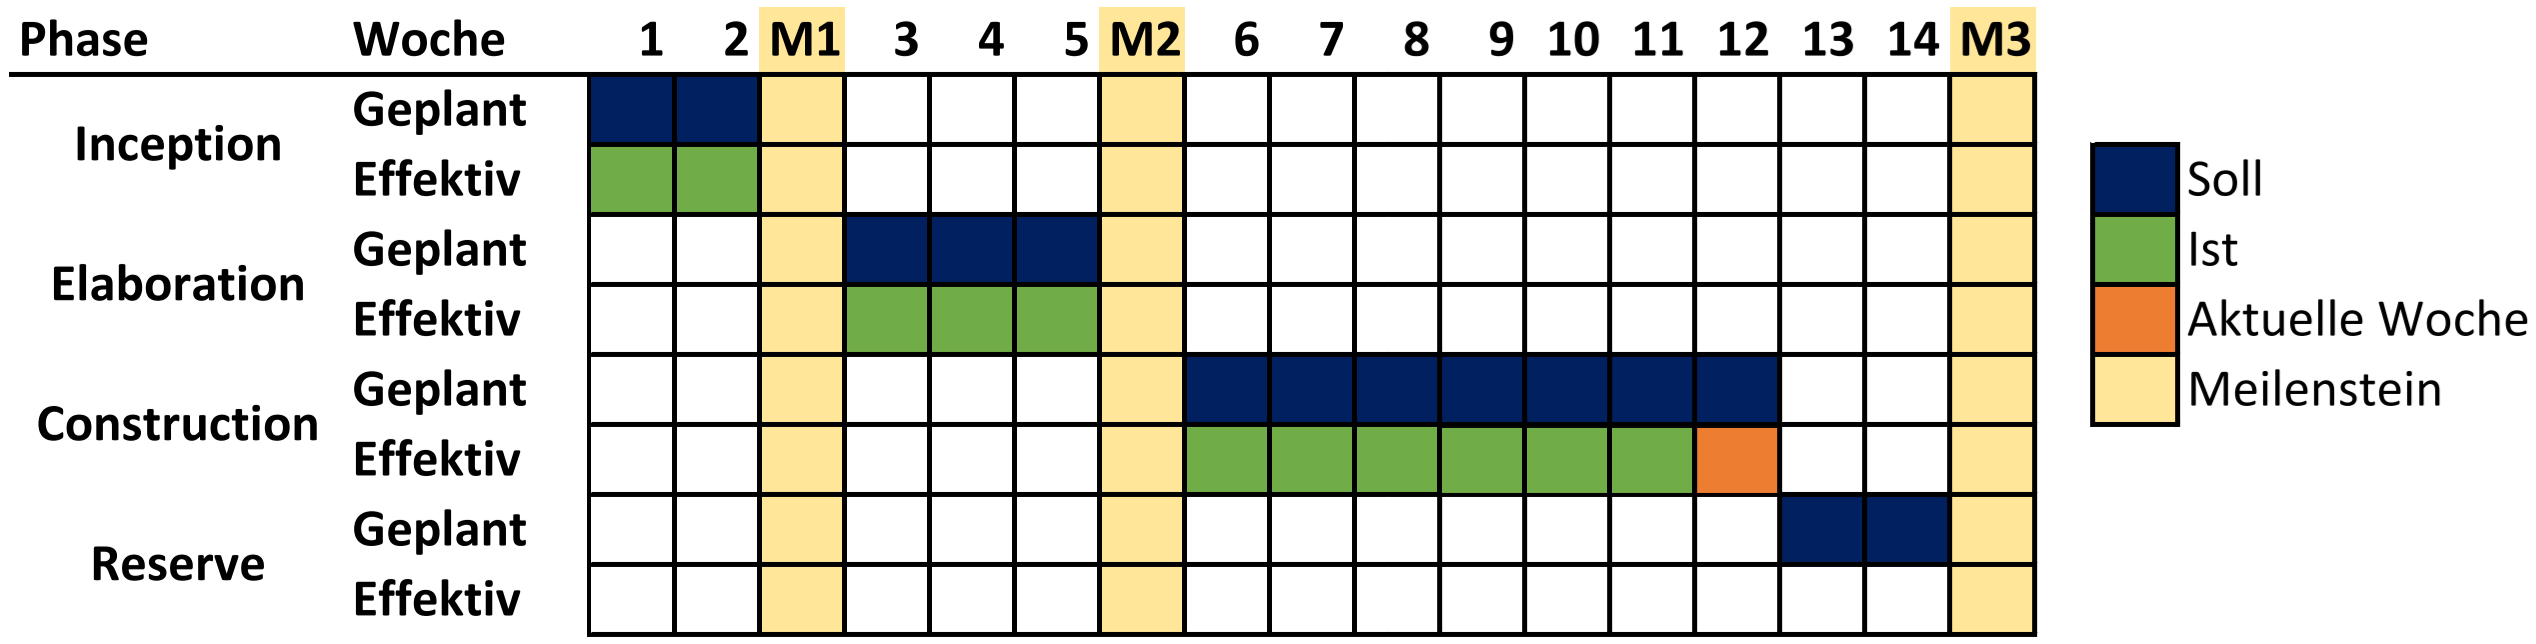
\includegraphics{Grobzeitplan_14.05.2017}
  \caption{Grobzeitplan Stand: 14.05.2017}
\end{figure}

\subsection{Methodik}


\subsection{Detaillierter Projektplan}\label{detaillierter-projektplan}
\begin{longtabu} to \textwidth { | l | l | X[l] | l | l | }
\hline
\textbf{Phase} & \textbf{Nr.} & \textbf{Arbeitspaket} & \textbf{Soll} & \textbf{Ist} \\\hline
\endhead

\multicolumn{5}{| l |}{ \textbf{Inception} }\\\hline
 & A-01 & Ausgangslage schildern & 5,0 h & 1,0 h \\\hline
 & A-02 & Projektidee beschreiben & 5,0 h & 2,0 h \\\hline
 & A-03 & Kundennutzen analysieren & 5,0 h & 3,0 h \\\hline
 & A-04 & Stand der Technik & 5,0 h & 1,5 h \\\hline
 & A-05 & Konkurenzanalyse & 5,0 h & 3,0 h \\\hline
 & A-06 & Hauptablauf aufzeigen & 5,0 h & 4,0 h \\\hline
 & A-07 & Weitere Anforderungen definieren & 5,0 h & 2,0 h \\\hline
 & A-08 & Ressource beschreiben & 5,0 h & 1,0 h\\\hline
 & A-09 & Projektidee beschreiben & 5,0 h & 6,0 h\\\hline
 & A-10 & Risiken beschreiben & 5,0 h & 0,5h \\\hline
 & A-11 & Grobplanung erstellen & 5,0 h & 3,5 h\\\hline
 & A-12 & Wirtschaftlichkeitsanalyse & 5,0 h & 6,0 h\\\hline
 & A-13 & Projektskizze erstellen (inkl. Präsentation) & 5,0 h & 10,0 h\\\hline
 & A-14 & Entwicklungsumgebung (inkl. Azure, DB) und Projekt aufsetzen für Backend & 10,0 h & 10,0 h\\\hline
 & A-15 & Entwicklungsumgebung und Projekt aufsetzen für Android App & 10,0 h & 11,0 h\\\hline
Total Phase: & 15 & & 85,0 h & 61,0 h\\\hline
\multicolumn{5}{| l |}{ }\\\hline

\multicolumn{5}{| l |}{ \textbf{Elaboration} }\\\hline
 & B-01 & Projekmanagement organisieren & 5,0 h & 6,0 h\\\hline
 & B-02 & Anwendungsfalldiagramm zeichnen & 5,0 h & 0,5 h \\\hline
 & B-03 & Domänenmodell erstellen & 5,0 h & 6,0 h\\\hline
 & B-04 & Architektur beschreiben & 5,0 h & 4,0 h \\\hline
 & B-05 & Zusätzliche Spezifikationen beschreiben & 5,0 h & 7,0 h \\\hline
 & B-06 & System Sequenzdiagramm zeichnen & 5,0 h & 2,5 h \\\hline
 & B-07 & Glossar erstellen & 5,0 h & 0,25 h \\\hline
 & B-08 & Anwendungsfall 1 beschreiben & 1,0 h & 1,0 h \\\hline
 & B-09 & Anwendungsfall 2 beschreiben & 0,5 h & 0,5 h \\\hline
 & B-10 & Anwendungsfall 3 beschreiben & 0,5 h & 0,5 h \\\hline
 & B-11 & Anwendungsfall 4 beschreiben & 0,5 h & 0,5 h \\\hline
 & B-12 & Anwendungsfall 5 beschreiben & 0,5 h & 0,5 h \\\hline
 & B-13 & Anwendungsfall 6 beschreiben & 0,5 h & 0,5 h\\\hline
 & B-14 & Analysedokument erstellen (inkl. Präsentation) & 6,5 h & 15,0 h\\\hline
 & B-15 & Erste Implementierungen an der Web API & 10 h & 20,0 h\\\hline
 & B-16 & Einarbeiten in Android SDK. Erste Implementierung an der Android App & 15 h & 24,0 h\\\hline
Total Phase: & 16 & & 70,0 h & 82,25 h\\\hline
\multicolumn{5}{| l |}{ }\\\hline

\multicolumn{5}{| l |}{ \textbf{Construction} }\\\hline
 & C-01 & Projekmanagement nachtragen & 1,0 h & 1,5 h \\\hline
 & C-02 & UC 1 Liste der verfügbaren Touren & 5,0 h & 6,0 h \\\hline
 & C-03 & UC 1 Starten einer Tour & 6,0 h & 5,5 h \\\hline
 & C-04 & UC 2 Lokalisieren des Benutzers & 6,0 h & 6,0 h \\\hline
 & C-05 & UC 2 Anzeigen des Benutzers auf der Karte & 4,0 h & 4,5 h \\\hline
 & C-06 & UC 3 Foto machen & 4,0 h & \\\hline
 & C-07 & UC 4 Prüfen der Geo-Koordinaten des Fotos & 6,0 h & \\\hline
 & C-08 & UC 5 Besuchen des nächsten Punktes & 6,0 h & 5,5 h \\\hline
 & C-09 & UC 6 Auslesen der Tourdaten & 5,0 h & \\\hline
 & C-10 & UC 6 Anzeigen der Tourdaten & 4,0 h & \\\hline
 & C-11 & UI gestalten & 8,0 h & 10,0\\\hline
 & C-12 & Designdokumentation erstellen & 28,0 h & 30,0 h \\\hline
 & C-13 & Systemtests durchführen & 12,0 h & \\\hline
 & C-14 & Schlussdokumentation erstellen & 10,0 h & \\\hline
 & C-15 & Benutzeranleitung schreiben & 8,0 h & 8,0\\\hline
Total Phase: & 15 & & 103,0 h & \\\hline
\end{longtabu}


\newpage
\subsection{Enteilung Arbeitspakete}\label{enteilung-arbeitspakete}
\begin{longtabu} to \textwidth { | l | l | l | X[l] | }
\hline
\textbf{Wer} & \textbf{Iteration} & \textbf{Paket} & \textbf{Beschreibung} \\\hline
\endhead

Alle                         & 1,2,3,4 & C-01 & Projekmanagement nachtragen \\\hline
Alle                         & 1,2,3,4 & C-11 & UI gestalten \\\hline
Andi, Benjamin, Josef        & 1       & C-02 & UC 1 Liste der verfügbaren Touren \\\hline
Nicolas, Raffaele            & 1       & C-03 & UC 1 Starten einer Tour \\\hline
Andi, Benjamin               & 2       & C-04 & UC 2 Lokalisieren des Benutzers \\\hline
Benjamin, Josef              & 2       & C-05 & UC 2 Anzeigen des Benutzers auf der Karte \\\hline
Raffaele, Andi               & 2       & C-08 & UC 5 Besuchen des nächsten Punktes \\\hline
Benjamin, Josef              & 3       & C-06 & UC 3 Foto machen \\\hline
Josef, Nicolas               & 3       & C-07 & UC 4 Prüfen der Geo-Koordinaten des Fotos \\\hline
Nicolas, Raffaele            & 3       & C-09 & UC 6 Auslesen der Tourdaten \\\hline
Raffaele, Andi               & 3       & C-10 & UC 6 Anzeigen der Tourdaten \\\hline
Alle                         & 3       & C-12 & Designdokumentation erstellen \\\hline
Josef, Benjamin              & 4       & C-13 & Systemtests durchführen \\\hline
Alle                         & 4       & C-14 & Schlussdokumentation erstellen \\\hline
Andi, Nicolas, Raffaele      & 4       & C-15 & Benutzeranleitung schreiben \\\hline
\end{longtabu}

\subsubsection{Übersicht nach Kategorie}

\begin{longtabu} to \textwidth { | X[l] | l | l | l | l | l | l | l | l | l | l | }
\hline
\textbf{Person} & \begin{turn}{90}\textbf{Infrastruktur}\end{turn} & \begin{turn}{90}\textbf{Dokumentation}\end{turn} & \begin{turn}{90}\textbf{Analyse/Design}\end{turn} & \begin{turn}{90}\textbf{Frontend}\end{turn} & \begin{turn}{90}\textbf{Backend}\end{turn} & \begin{turn}{90}\textbf{Testing}\end{turn} & \begin{turn}{90}\textbf{Administratives}\end{turn} & \begin{turn}{90}\textbf{Meetings}\end{turn} & \begin{turn}{90}\textbf{Präsentationen}\end{turn} & \begin{turn}{90}\textbf{Total}\end{turn} \\\hline
\endhead

Josef Erben           & 5h & 3h  & 20h & 40h & 0h  & 10h & 10h & 10h & 8h & 106h\\\hline
Andi Saurer           & 3h & 25h & 12h & 35h & 0h  & 2h  & 5h  & 10h & 8h & 100h\\\hline
Raffaele Bof          & 2h & 3h  & 15h & 35h & 0h  & 2h  & 25h & 10h & 8h & 100h\\\hline
Nicolas Loth          & 10h & 15h & 10h & 0h & 20h & 10h & 7h & 10h & 8h & 100h    \\\hline
Benjamin Schneidinger & 2h & 42h & 10h & 0h  & 40h & 3h  & 5h  & 10h & 8h & 120h\\\hline
Total                 &    &     &     &     &     &     &     &     &    &     \\\hline
\end{longtabu}

\subsection{Abweichungen}\label{abweichungen}


\subsection{Rückblick}\label{rueckblick}
Die Durchführung des Projektes war für alle Teammitglieder eine positive Erfahrung. Trotz der grossen 
Herausforderung, die dieses Projekt darstellte, wurde es durch gute Kooperation und Koordination 
rechtzeitig und in guter Qualität fertiggestellt.
Jedes einzelne Teammitglied hat grossen Einsatz gezeigt und ist anderen bei Problemen unterstützend 
zur Seite gestanden. Aufgrund des straffen Zeitplans war der Wissensaustausch zwischen dem Frontend- 
und dem Backend-Team leider sehr gering. 
Für alle war die Entwicklung einer Mobile App für Android etwas Neues, daher musste das Wissen zuerst 
aufgebaut werden. Da im Team jedoch genügend erfahrene Entwickler vorhanden sind, konnten diese 
Wissenslücken rasch und effizient gefüllt werden. Ebenfalls sind sich die Teammitglieder persönlich 
etwas näher gekommen und konnten Erfahrungen aus dem Leben und der Arbeit austauschen.

\newpage
\subsection{Risiken}\label{risiken}
\begin{longtabu} to \textwidth { | l | X[l] | l | l | X[l] | }
\hline
\textbf{Nr.} & \textbf{Risiko} & \textbf{Auswirkung} & \textbf{Wahrscheinlichkeit} & \textbf{Massnahmen} \\\hline
\endhead

1 & Schutz der gespeicherten Daten durch unautorisierte Zugriffe & Schwerwiegend & Hoch & Verwendung von Sicherheitsmassnahmen auf dem heutigen Stand der Technik\\\hline
2 & Hohe Kosten für Anwender aufgrund der Verwendung durch Kartenmaterial & Mittel & Hoch & Offlinespeicherung des Kartenmaterials\\\hline
3 & Fehlendes Wissen in der Entwicklung von Mobile Apps & Mittel & Mittel & Aneignen des Wissens mittels Online-Tutorials und Wissensaustausch zwischen Gruppenmitgliedern\\\hline
4 & Höhere Komplexität durch Einbinden von Drittanbieter Software & Gering & Mittel & Auf die Einbindung von Software von Drittanbietern möglichst verzichten\\\hline
5 & Smartphone GPS-Koordinaten ungenau & Gering & Mittel & Die App für Geräte mit zu geringer GPS-Genauigkeit nicht freigeben\\\hline
\st{6} & \st{Keine öffentlichen Karten-API verfügbar} & \st{Schwerwiegend} & \st{Sehr gering} & Entsprechendes Kartenmaterial ist von Google verfügbar\\\hline
\end{longtabu}
